\documentclass[10pt, a4paper]{article}
\usepackage{triada}

\graphicspath{{eps/}{png/}}

\renewcommand{\ell}{\mathcal{E}}

\usepackage{delim}
\usepackage{float}
\usepackage{subfigure}
\usepackage[subfigure]{ccaption}

\begin{document}
\thispagestyle{empty}

\begin{center}
\ \vspace{-3cm}


\includegraphics[width=0.5\textwidth]{msu.eps}\\
{\scshape Московский государственный университет имени М.~В.~Ломоносова}\\
Факультет вычислительной математики и кибернетики\\
Кафедра системного анализа



%\vspace{5cm}
\vfill
{\LARGE Лабораторная работа}

\vspace{1cm}

{\huge\bfseries <<Оценка влияния государственной энергетической политики на потенциал экономического роста России>>}
\end{center}

\vspace{2cm}

\begin{flushright}
  \large
  \textit{Студент 415 группы}\\
  Д.~И.~Степенский

  \vspace{5mm}

  \textit{Руководитель практикума}\\
  к.\,ф.-м.\,н., асс. А.~В.~Рудева
\end{flushright}

\vfill

\begin{center}
Москва, 2012
\end{center}

\newpage

\tableofcontents

\newpage

\section{Постановка задачи}
Требуется построить и проанализировать зависимости от доли экспорта в выпуске нефтегазовой отрасли следующих макроэкономических показателей:
\begin{itemize}
\item темп роста цен;
\item темп роста производства;
\item параметр неэффективности;
\item доля налогов в добавленной стоимости электроэнергетики;
\item доля зарплаты и распределяемой прибыли в добавленной стоимости НГК;
\item доля потребления населения к ВВП;
\item доля государственных расходов в ВВП;
\item доля добавленной стоимости 1-го сектора в ВВП;
\item доля добавленной стоимости 2-го сектора в ВВП;
\item доля добавленной стоимости 3-го сектора в ВВП;
\item отношение инвестиций во 2-ой сектор к выпуску 2-го сектора;
\item отношение инвестиций в 3-ий сектор к выпуску 3-го сектора;
\end{itemize}
а также объяснить влияние параметра неэффективности на макроэкономические модели.

\section{Графики и анализ}
Ниже на всех рисунках, кроме \subref{uneffectiveness} синяя линия является графиком, отвечающим модели без учёта неэффективности, красная --- с учётом. В \subref{uneffectiveness} синяя линия ---  собственно значение неэффективности.
\begin{figure}[H]
\centering
\contsubbottom[Темп роста цен.]{
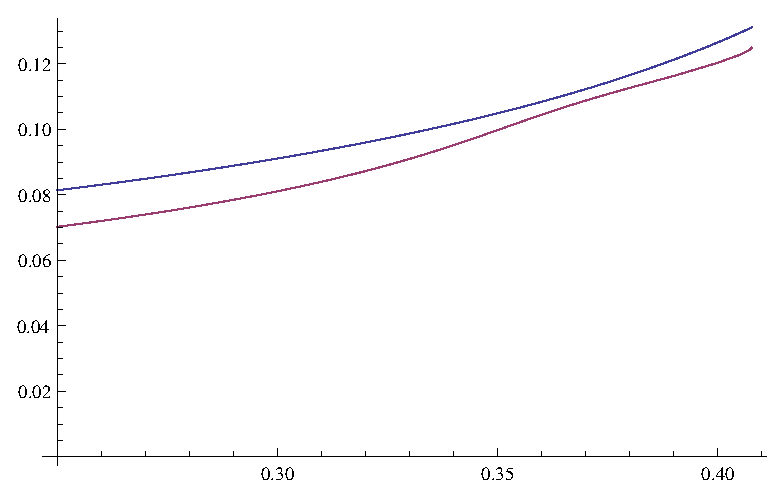
\includegraphics[scale=0.5]{1.eps}
}
\contsubbottom[Темп роста производства.]{
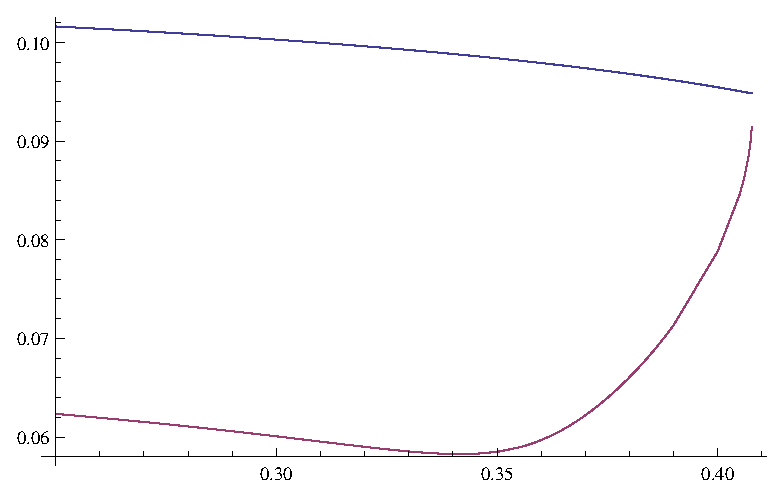
\includegraphics[scale=0.5]{2.eps}
}
\end{figure}
\begin{figure}[H]
\centering
\contsubbottom[Параметр неэффективности.]{
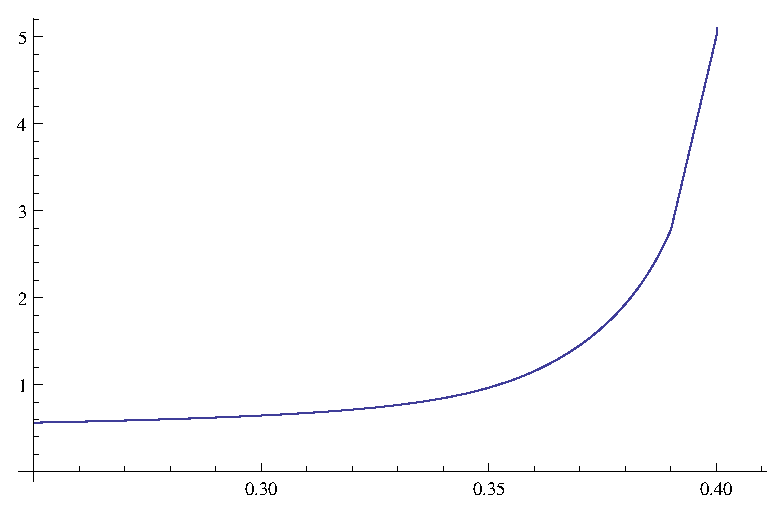
\includegraphics[scale=0.5]{3.eps}\label{uneffectiveness}
}
\contsubbottom[Доля налогов в добавленной стоимости электроэнергетики.]{
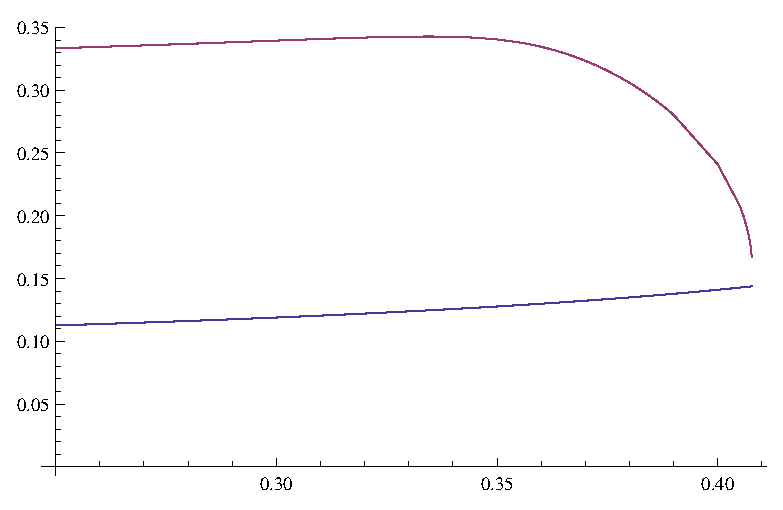
\includegraphics[scale=0.5]{4.eps}
}
\end{figure}
\begin{figure}[H]
\centering
\contsubbottom[Доля зарплаты и распределяемой прибыли в добавленной стоимости НГК.]{
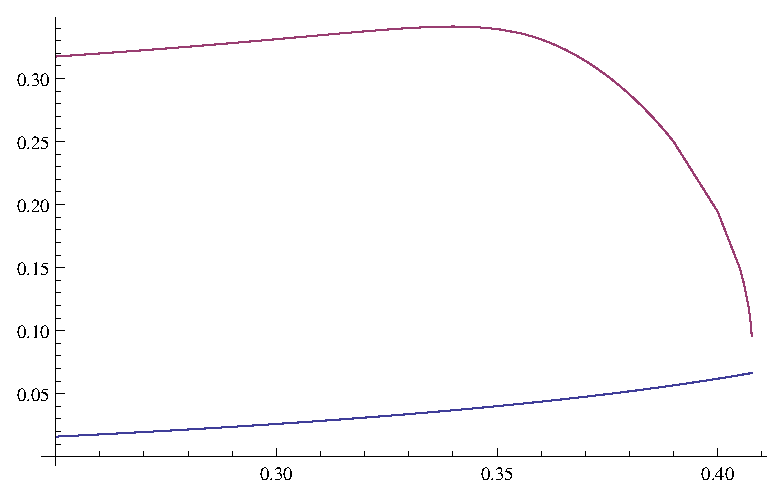
\includegraphics[scale=0.5]{5.eps}
}
\contsubbottom[Доля потребления населения к ВВП.]{
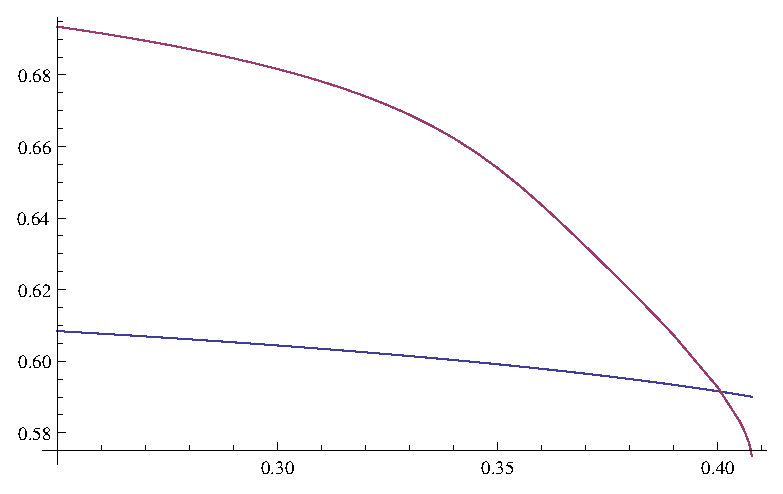
\includegraphics[scale=0.5]{6.eps}
}
\end{figure}
\begin{figure}[H]
\centering
\contsubbottom[Доля государственных расходов к ВВП]{
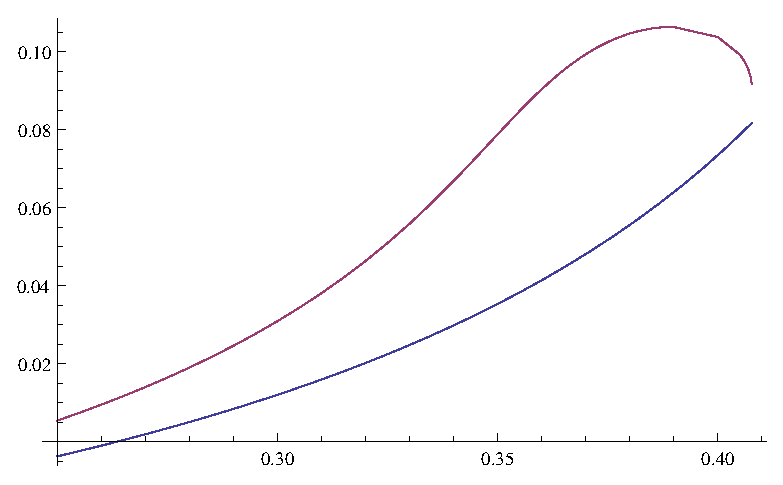
\includegraphics[scale=0.5]{7.eps}
}
\contsubbottom[Доля добавленной стоимости 1-го сектора в ВВП]{
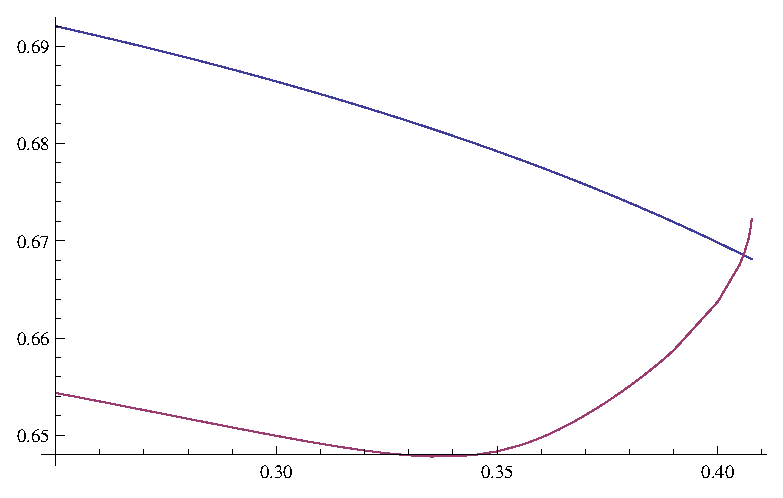
\includegraphics[scale=0.5]{8.eps}
}
\end{figure}
\begin{figure}[H]
\centering
\contsubbottom[Доля добавленной стоимости 2-го сектора в ВВП]{
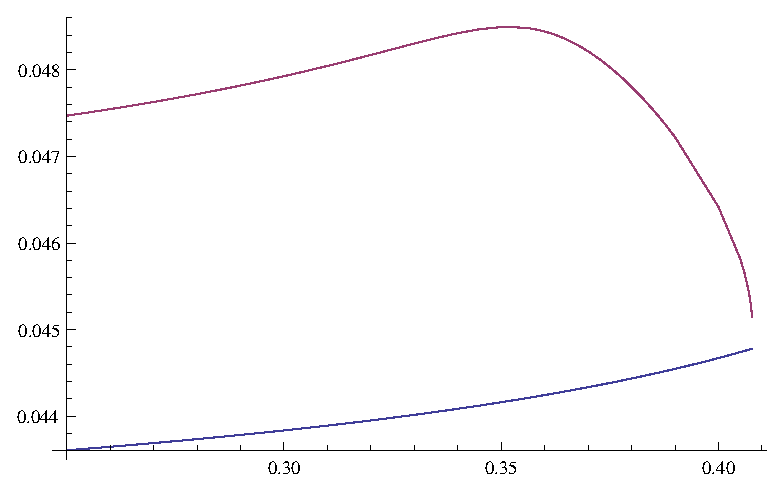
\includegraphics[scale=0.5]{9.eps}
}
\contsubbottom[Доля добавленной стоимости 3-го сектора в ВВП]{
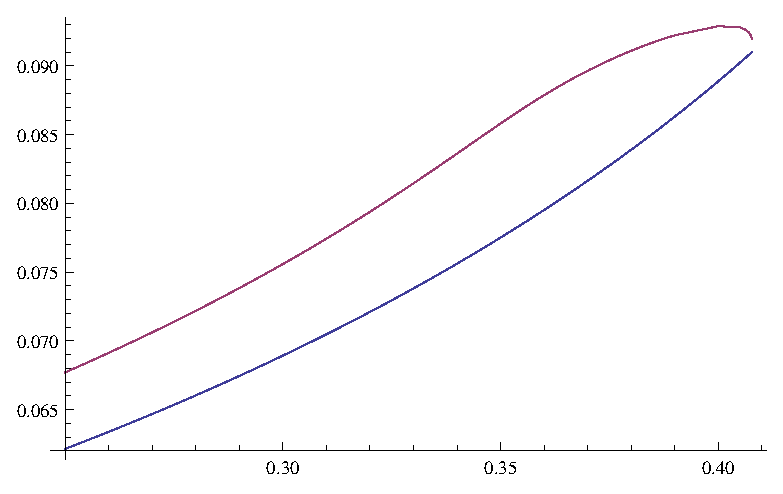
\includegraphics[scale=0.5]{10.eps}
}
\end{figure}
\begin{figure}[H]
\centering
\contsubbottom[Отношение инвестиций во 2-ой сектор к выпуску 2-го сектора.]{
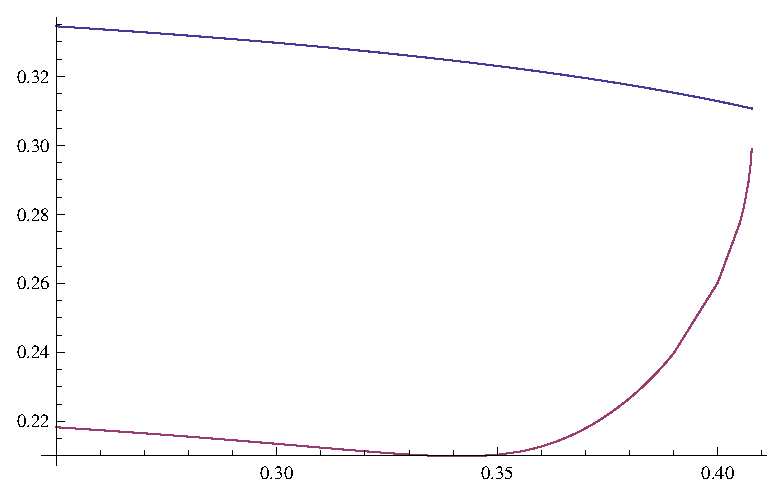
\includegraphics[scale=0.5]{11.eps}
}
\contsubbottom[Отношение инвестиций во 3-ий сектор к выпуску 3-го сектора.]{
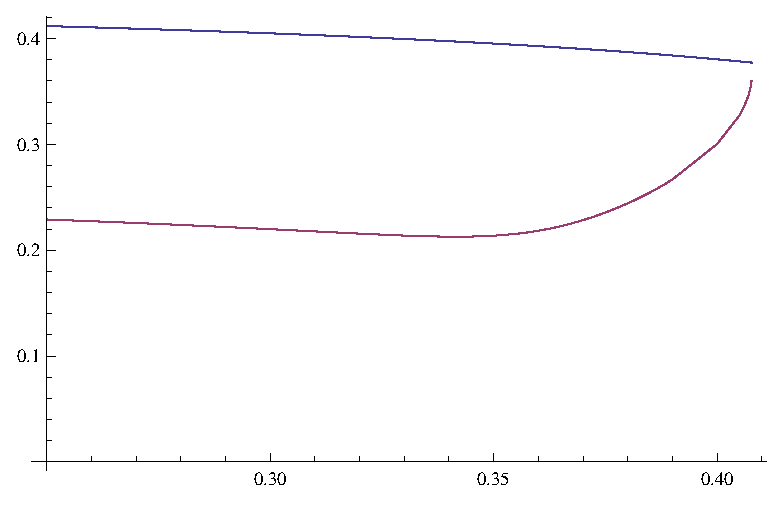
\includegraphics[scale=0.5]{12.eps}
}
\end{figure}

Нетрудно заметить, что на всех графиках второй модели происходит качественное изменение тенденций около значения доли экспорта третьей отрасли, равного $0.35$, в частности, начинает быстро расти параметр неэффективности.

Кроме увеличения неэффективности происходят и другие изменения. Темпы роста производства перестают падать и более того, начинают расти с увеличивающейся скоростью. 

Доля добавленной стоимости первого сектора в ВВП начинает расти, а доля второго, соответственно, убывать, доля же третьего сектора растёт почти линейно практически на всём промежутке измерений.

Доли налогов в добавленной стоимости и зарплаты и распределяемой прибыли резко падают после значения доли экспорта $0.35$.

Поведение графиков показывает важность учёта неэффективности при использовании различных моделей: при учёте этого параметра многие характеристики модели качественно меняются. Лишь незначительное количество характеристик: характеристики третьей отрасли, темп роста цен --- не показывают значительных качественных изменений при смене модели, из чего можно заключить, что для их измерения можно пользоваться более простой моделью без учёта параметра неэффективности.

Стоит также заметить, что до значения параметра $w_3=0.35$ можно характеристики обеих моделей показывают одинаковые тенденции, то есть, например, доли государственных расходов относительно ВВП растут с одинаковой скоростью. Таким образом, прогнозировать темпы роста до данного переходного значения параметра можно даже с помощью более простой модели.
\end{document}